% Created by tikzDevice version 0.12.3.1 on 2022-03-31 14:18:16
% !TEX encoding = UTF-8 Unicode
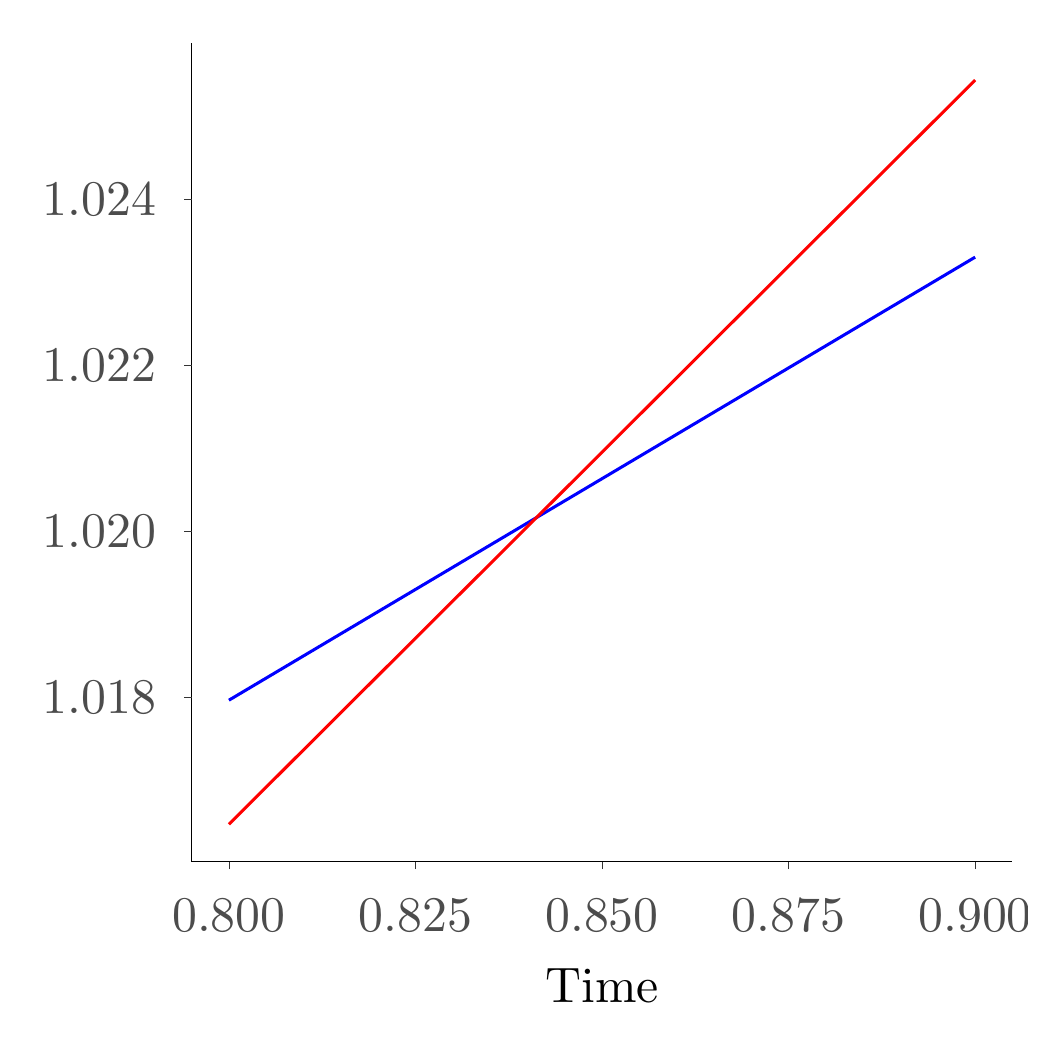
\begin{tikzpicture}[x=1pt,y=1pt]
\definecolor{fillColor}{RGB}{255,255,255}
\path[use as bounding box,fill=fillColor,fill opacity=0.00] (0,0) rectangle (361.35,361.35);
\begin{scope}
\path[clip] (  0.00,  0.00) rectangle (361.35,361.35);
\definecolor{drawColor}{RGB}{255,255,255}
\definecolor{fillColor}{RGB}{255,255,255}

\path[draw=drawColor,line width= 0.1pt,line join=round,line cap=round,fill=fillColor] (  0.00,  0.00) rectangle (361.35,361.35);
\end{scope}
\begin{scope}
\path[clip] ( 59.24, 60.04) rectangle (355.85,355.85);
\definecolor{fillColor}{RGB}{255,255,255}

\path[fill=fillColor] ( 59.24, 60.04) rectangle (355.85,355.85);
\definecolor{drawColor}{RGB}{0,0,255}

\path[draw=drawColor,line width= 1.1pt,line join=round] ( 72.72,118.33) --
	(342.37,278.43);
\definecolor{drawColor}{RGB}{255,0,0}

\path[draw=drawColor,line width= 1.1pt,line join=round] ( 72.72, 73.49) --
	(342.37,342.40);
\end{scope}
\begin{scope}
\path[clip] (  0.00,  0.00) rectangle (361.35,361.35);
\definecolor{drawColor}{RGB}{0,0,0}

\path[draw=drawColor,line width= 0.1pt,line join=round] ( 59.24, 60.04) --
	( 59.24,355.85);
\end{scope}
\begin{scope}
\path[clip] (  0.00,  0.00) rectangle (361.35,361.35);
\definecolor{drawColor}{gray}{0.30}

\node[text=drawColor,anchor=base east,inner sep=0pt, outer sep=0pt, scale=  1.80] at ( 46.49,113.38) {1.018};

\node[text=drawColor,anchor=base east,inner sep=0pt, outer sep=0pt, scale=  1.80] at ( 46.49,173.38) {1.020};

\node[text=drawColor,anchor=base east,inner sep=0pt, outer sep=0pt, scale=  1.80] at ( 46.49,233.37) {1.022};

\node[text=drawColor,anchor=base east,inner sep=0pt, outer sep=0pt, scale=  1.80] at ( 46.49,293.36) {1.024};
\end{scope}
\begin{scope}
\path[clip] (  0.00,  0.00) rectangle (361.35,361.35);
\definecolor{drawColor}{gray}{0.20}

\path[draw=drawColor,line width= 0.1pt,line join=round] ( 56.49,119.58) --
	( 59.24,119.58);

\path[draw=drawColor,line width= 0.1pt,line join=round] ( 56.49,179.58) --
	( 59.24,179.58);

\path[draw=drawColor,line width= 0.1pt,line join=round] ( 56.49,239.57) --
	( 59.24,239.57);

\path[draw=drawColor,line width= 0.1pt,line join=round] ( 56.49,299.56) --
	( 59.24,299.56);
\end{scope}
\begin{scope}
\path[clip] (  0.00,  0.00) rectangle (361.35,361.35);
\definecolor{drawColor}{RGB}{0,0,0}

\path[draw=drawColor,line width= 0.1pt,line join=round] ( 59.24, 60.04) --
	(355.85, 60.04);
\end{scope}
\begin{scope}
\path[clip] (  0.00,  0.00) rectangle (361.35,361.35);
\definecolor{drawColor}{gray}{0.20}

\path[draw=drawColor,line width= 0.1pt,line join=round] ( 72.72, 57.29) --
	( 72.72, 60.04);

\path[draw=drawColor,line width= 0.1pt,line join=round] (140.13, 57.29) --
	(140.13, 60.04);

\path[draw=drawColor,line width= 0.1pt,line join=round] (207.55, 57.29) --
	(207.55, 60.04);

\path[draw=drawColor,line width= 0.1pt,line join=round] (274.96, 57.29) --
	(274.96, 60.04);

\path[draw=drawColor,line width= 0.1pt,line join=round] (342.37, 57.29) --
	(342.37, 60.04);
\end{scope}
\begin{scope}
\path[clip] (  0.00,  0.00) rectangle (361.35,361.35);
\definecolor{drawColor}{gray}{0.30}

\node[text=drawColor,anchor=base,inner sep=0pt, outer sep=0pt, scale=  1.80] at ( 72.72, 34.90) {0.800};

\node[text=drawColor,anchor=base,inner sep=0pt, outer sep=0pt, scale=  1.80] at (140.13, 34.90) {0.825};

\node[text=drawColor,anchor=base,inner sep=0pt, outer sep=0pt, scale=  1.80] at (207.55, 34.90) {0.850};

\node[text=drawColor,anchor=base,inner sep=0pt, outer sep=0pt, scale=  1.80] at (274.96, 34.90) {0.875};

\node[text=drawColor,anchor=base,inner sep=0pt, outer sep=0pt, scale=  1.80] at (342.37, 34.90) {0.900};
\end{scope}
\begin{scope}
\path[clip] (  0.00,  0.00) rectangle (361.35,361.35);
\definecolor{drawColor}{RGB}{0,0,0}

\node[text=drawColor,anchor=base,inner sep=0pt, outer sep=0pt, scale=  1.80] at (207.55,  9.00) {Time};
\end{scope}
\end{tikzpicture}
